\section{Apache Kafka. Физическая организация партиций. Автоматическое распределение сообщений. Хеширование ключей сообщений. Репликация данных.}

Партиция делится на сегменты, которые хранятся в отдельной директории на диске.

Директория состоит из файлов:
\begin{itemize}
    \item Сегментов (*.log)
    \item Разряженного индекса оффсетов (*.index)
    \item Разряженного индекса временных меток (*.timeindex)
\end{itemize}

Размер сегмента ограничен и контролируется 
двумя параметрами — log.segment.bytes, 
log.segment.ms .

АКТИВЕН только один сегмент —
в него записываются данные.

Сегмент можно удалить только в том случае, 
если он был предварительно закрыт.

Изменять нельзя.

Данные находятся в бинарном виде.

Index хранит пары: относительный оффсет записи в сегменте – позиция в .log 
файле.

Так как данные упорядоченные, можно хранить значения только для 
некоторых (экономия памяти), а остальные находить линейным чтением

TimeIndex - то же самое, но по времени.

\subsection*{Сообщения}

\D{
    Сообщение содержит ключ и значение.

    Ключ и значение сериализуются и отправляются к брокеру.

    Распределение по партициям зависит от ключа:
    \begin{itemize}
        \item message.key is null => auto
        \item message.key is not null => hash
    \end{itemize}
}

Сообщения с одинаковым ключем попадут в одну партицию.

\begin{figure}[ht]
	\centering
	\begin{minipage}[b]{0.65\textwidth}
		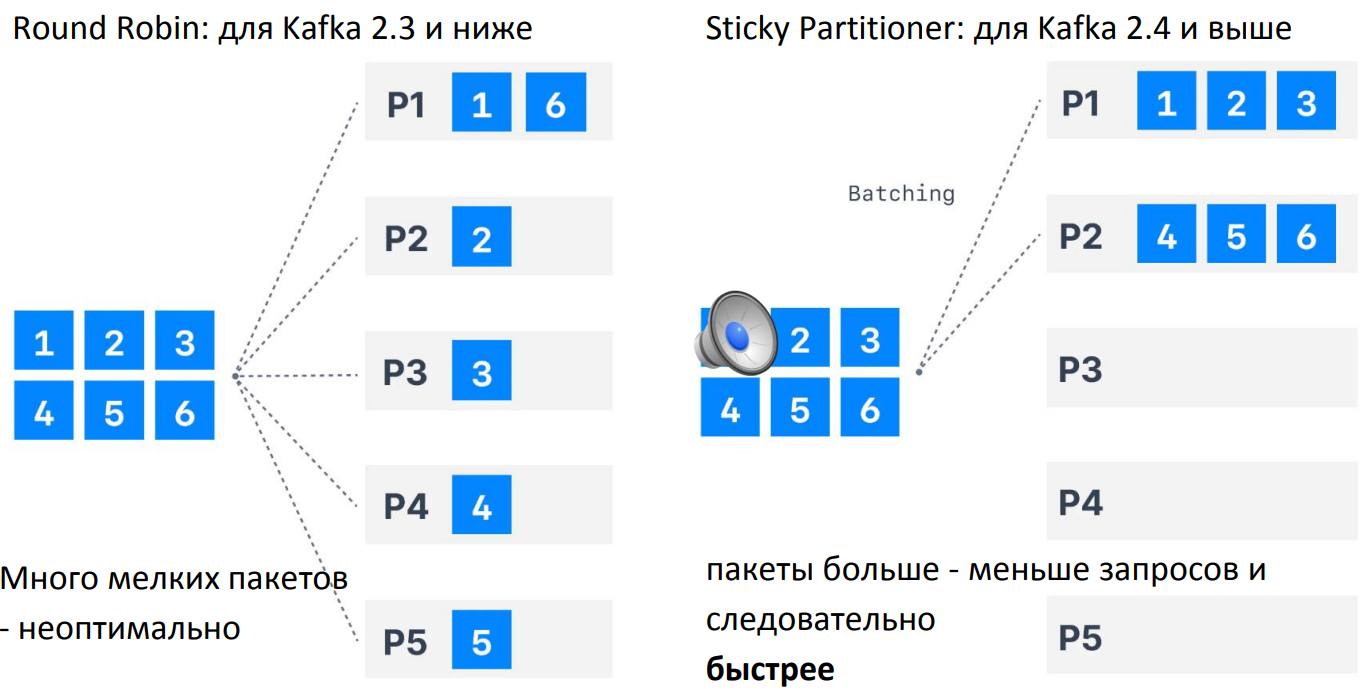
\includegraphics[width=\textwidth]{images/part.png}
        \caption{Автоматическое распределение сообщений}
	\end{minipage}
\end{figure}


\subsubsection*{Репликация данных}

\D{
    Репликация - копирование сообщений нескольким брокерам.

    Противостоит сбоям.
}

Лидер и синхронизированные реплики.
Если лидер падает – реплика станет лидером если превышены:
\begin{itemize}
    \item replica.lag.max.messages – допустимая разница между оффсетом реплики и 
    лидера
    \item replica.lag.time.max.ms - интервал времени, в течение которого каждая реплика 
    должна запросить у лидера свой статус
\end{itemize}


